\documentclass[12pt]{article}
%--------------------   start of the 'preamble'
%
\usepackage{graphicx,amssymb,amstext,amsmath,color}
\usepackage[margin=2cm]{geometry}
\usepackage{abstract}
\usepackage{setspace}
\usepackage[footnotesize,bf]{caption}

% TABLE
\usepackage{multicol,hhline,colortbl,multirow}
\usepackage{braket}
\usepackage{siunitx}
\usepackage{hyperref}
\usepackage{authblk}
\usepackage{siunitx}
\usepackage{adjustbox}
\usepackage{mathrsfs}
%%\usepackage[sort&compress]{natbib}
%%\bibpunct{(}{)}{,}{a}{, }{;}
%
\usepackage[sort&compress]{natbib}
\bibpunct{[}{]}{,}{s}{}{;}


\definecolor{gray}{gray}{0.8}
\def\mobunits{\square\centi\meter\per\volt\per\second}
\def\gcm{\gram\per\cubic\centi\meter}
\def\ccg{\cellcolor{gray}}

\renewcommand{\labelitemii}{$\circ$}
\renewcommand{\bibname}{References}


\title{MorphCT Results - Fine Graining Comparison}
\author{Matthew Jones}
\date{\today}

\begin{document}
\maketitle

\section{Summary}

This document is an addendum to both the Voronoi Neighbour Analysis and the Neat P3HT results to consider the differences between the OrigFG and the NewFG results.

The centre-of-mass deviations from the CG morphology to the final chromophore positions after fine-graining are all located within 5~\AA, with the majority of chromophores around 2~\AA~away from their initial positions.

\subsection{CoM Deviations}

\begin{figure}[h!]\centering
	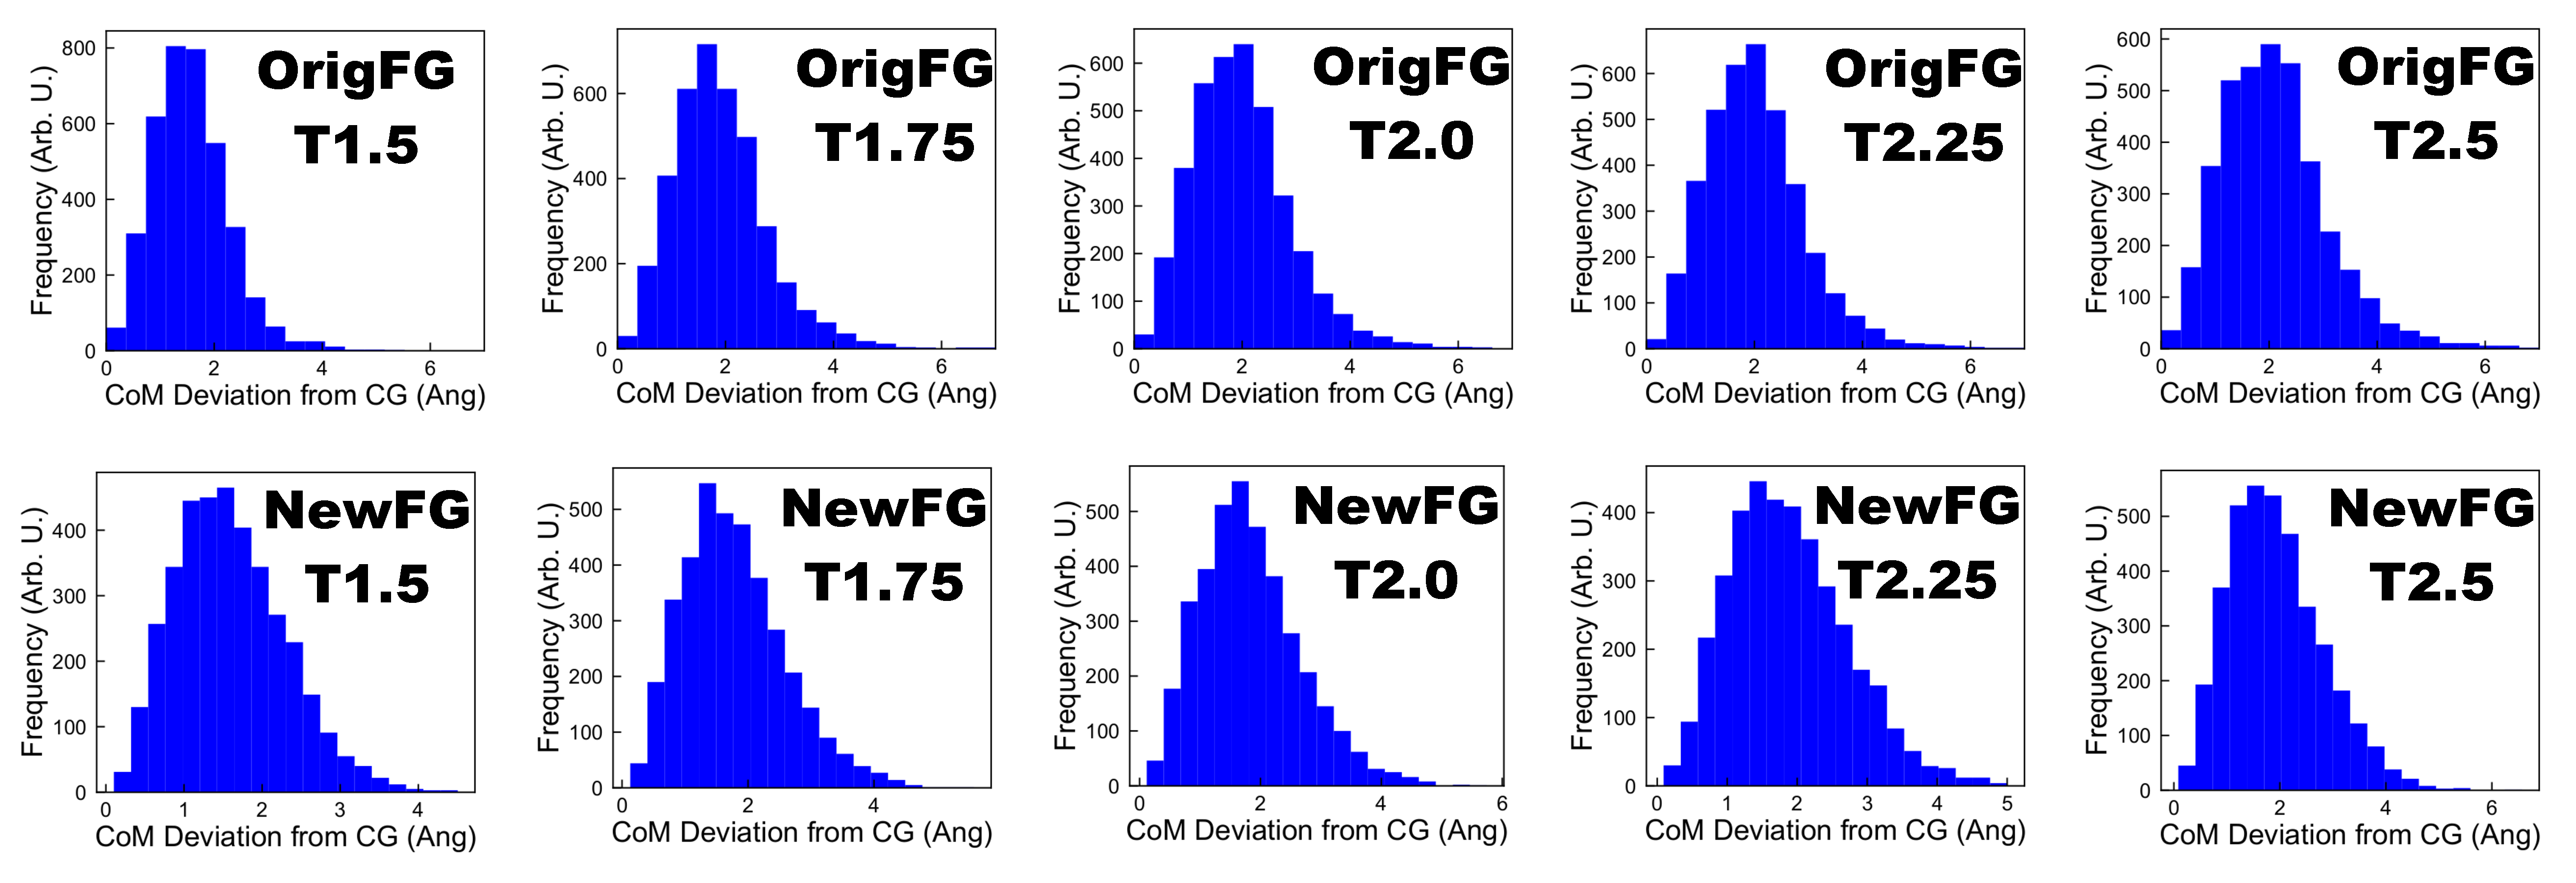
\includegraphics[width=\textwidth]{Figures/CoMDeviation.pdf}
    \caption{The distribution of physical deviations between the coarse-grained bead centre of mass describing the chromophore from the input and the resultant centre of mass of the chromophore after fine-graining.}
	\label{fig:Deviation}
\end{figure}

\bibliography{refs}
\bibliographystyle{unsrt}


\end{document}
